The sun is the primary source of energy for Earth, essential for photosynthesis in plants, which forms the basis of most food chains, and for driving the weather and climate systems that shape our environment. Its consistent radiation supports all life forms, regulates global temperatures, and influences fundamental ecological and biological processes that are vital for the Earth's diverse ecosystems. From the very outset of human life, the sun has been a subject of profound admiration, occupying a central role in various religious beliefs and was often synonym of an incomparably vast and potent source of energy. It was not until the beginning of the twentieth century that progress in particle physics allowed to unravel the secret of solar energy: nuclear fusion. It is the physical process where two light atomic nuclei merge to form a heavier nucleus, releasing significant energy as a result of mass-to-energy conversion. \newline 
The dream of achieving nuclear fusion in a laboratory to produce energy emerged shortly thereafter. In today's climate crisis, nuclear fusion is even more appealing because it does not emit carbon emissions, does not present the risk of a catastrophic meltdown and its fuel, hydrogen, is readily available. Since replicating the sun's core conditions on Earth, particularly the immense pressure, is not feasible, alternative approaches were searched. A look at the reaction cross-section of various pairs of light atoms shows that deuterium-tritium (D-T) fusion has the highest likelihood at the lowest temperature. These two hydrogen isotopes are hence the most favorable candidates for fusion; deuterium is naturally abundant, but tritium, which is radioactive and has a relatively short half-life, must be artificially produced. \newline

\begin{figure}[H]
	\centering
	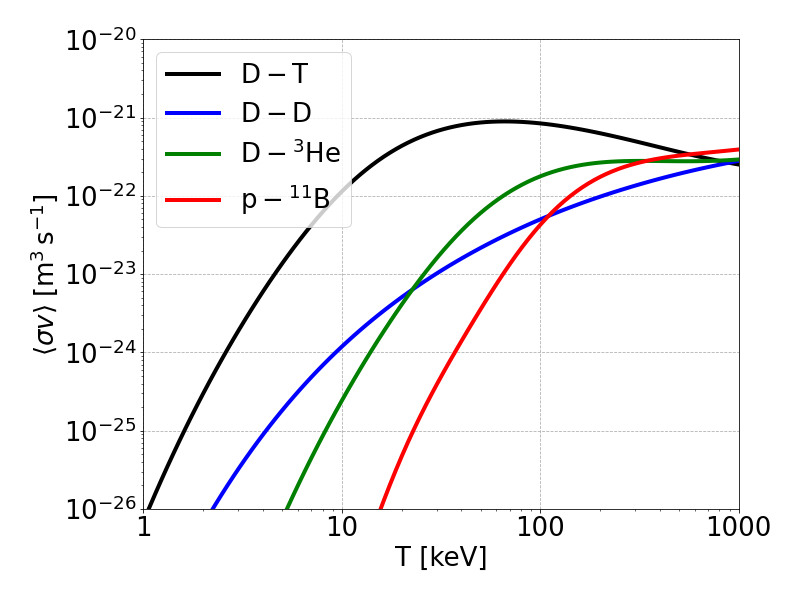
\includegraphics[width=0.62\textwidth]{schemes/fusion-reactivities.png}
	\caption{Fusion reaction cross-sections for the most promising pairs of light elements over plasma temperature.}
	\label{fig:Intro_fusionCrossSections}
\end{figure}

At such elevated temperatures, the binding energy is insufficient to maintain the cohesion of electrons and atomic nuclei, resulting in the formation of a state of matter known as plasma. Fundamentally, plasma is an ionized gas composed of positively charged nuclei and negatively charged electrons, which interact electromagnetically. 
\newline
Lawson's criterion\cite{Lawson1957} estimates the necessary plasma conditions to reach the break-even point, when fusion power exceeds heating and conduction losses. For D-T fusion, the triple product of density $n$, temperature $T$ and confinement time $\tau_E$ must exceed:
\begin{equation}
	\label{eq:LawsonCriterionDT}
	nT\tau_E > 10^{-21} \text{keV m}^{-3}\text{s}
\end{equation}
 
The reaction cross-section determines an optimal temperature of approximately 15-40 keV  (~150 millions °C) for fusion reactions, leading fusion reactor designs to focus on maximizing either of the two remaining parameters: density or confinement time. Inertial Confinement Fusion (ICF) seeks to compress dense fuel pellets for an extremely brief duration using high-powered lasers. Conversely, Magnetic Confinement Fusion (MCF) utilizes strong magnetic fields to sustain stable plasmas at relatively low densities. Both approaches have conducted promising experiments close to the break-even point. Within MCF, there are two primary designs: tokamaks, which use a toroidal chamber with an axisymmetric magnetic field, and stellarators, which use a twisted magnetic configuration to improve plasma confinement.
\newline

For MCF
Plasma heating
- Ohmic heating
- ICRH, ECRH, NBI

fusion gain Q as essential metric.

show diagram with all machines, scaling laws for fusion performance

The largest fusion experiment ITER, employing tokamak technology, is currently under construction in southern France by an international collaboration of seven member parties. At its full operation it is expected to achieve ignition, a state where the fusion reaction emits sufficiently radiation to maintain the plasma conditions. It requires a heat exhausts ten times higher than the break-even point and is a critical milestone for the development of future commercial fusion reactors. 

Introduce necessity for (electromagnetic) turbulent simulations (estimate cross-field transport, power exhaust,ELMs...)